 % !TeX spellcheck = en_US
\documentclass[french]{yLectureNote}

\title{Optique Géométrique}
\subtitle{Niveau 1}
\author{Paulhenry Saux}
\date{\today}
\yLanguage{Français}

\professor{C.Gatel}%christophe.gatel@cemes.fr : section B sillon 7

\usepackage{graphicx}%----pour mettre des images
\usepackage[utf8]{inputenc}%---encodage
\usepackage{geometry}%---pour modifier les tailles et mettre a4paper
%\usepackage{awesomebox}%---pour les boites d'exercices, de pbq et de croquis ---d\'esactiv\'e pour les TP de PC
\usepackage{tikz}%---pour deiffner + d\'ependance de chemfig
\usepackage{tkz-tab}
\usepackage{chemfig}%---pour deiffner formules chimiques
\usepackage{chemformula}%---pour les formules chimiques en \'equation : \ch{...}
\usepackage{tabularx}%---pour dimensionner automatiquement les tableaux avec variable X
\usepackage{awesomebox}%---Pour les boites info, danger et autres
\usepackage{menukeys}%---Pour deiffner les touches de Calculatrice
\usepackage{fancyhdr}%---pour les en-t\^ete personnalis\'ees
\usepackage{blindtext}%---pour les liens
\usepackage{hyperref}%---pour les liens (\`a mettre en dernier)
\usepackage{caption}%---pour la francisation de la l\'egende table vers Tableau
\usepackage{pifont}
\usepackage{array}%---pour les tableaux
\usepackage{lipsum}
\usepackage{yFlatTable}
\usepackage{multicol}
\newcommand{\Lim}[1]{\lim\limits_{\substack{#1}}\:}
\renewcommand{\vec}{\overrightarrow}
\begin{document}
\setcounter{chapter}{1}
	\chapter{Réflexion et réfraction}
	\section{Réflexion}
	\subsection{Définitions}
	\begin{itemize}
	 \item Le premier milieu est le milieu incident,
	 \item Si la lumière ne peut rentrer dans le deuxième milieu, il est hachuré
	 \item Direction de référence : normale au 2e milieu au point d'arrivée du rayon incident sur la surface. La lumière arrive en faisant un ange défini par rapport à la normale. ($0<\alpha<\frac{\pi}{2}$)
	 \item Plan d'incidence : Plan contenant la normale et le rayon incident, perpendiculaire à la surface.
	\end{itemize}
	\subsection{Loi de la réflexion}
	\warningInfo{Propriétés}{le rayon est réflchi :
	\begin{itemize}
\item dans le m\^eme pan d'incidence
\item repart avec le m\^eme angle par rapport à la normale à l'angle d'incidence.
	\end{itemize}}


	\section{Réfraction}
	On considère un dioptre séparant 2 milieux transparents (incidnets et réfractant). .
\warningInfo{Propriétés}{
\begin{itemize}
 \item Le rayon réfracté reste dans le plan d'incidence.
 \item On a $n_1\sin(i_1) = n_2 \sin(i_2)$
\end{itemize}
}
On remarque donc que si $n_i$ augmente, $i_n$ diminue.
On remarque donc que si $n_i$ diminue, $i_n$ augmente, et il peut y avoir réflexion totale.

	\subsection{Analyse}
	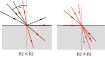
\includegraphics{fig2}
	\subsubsection{Si $n_2 > n_1$}
	Si $n_2 > n_1$, on dit que le milieu 2 est plus réfreingent et le rayon réfracté se rapproche de la normale.

	Cas extrèmes : $i_1 = 0 \Rightarrow i_2 = 0$ et $i_1 = \pi/2 \Rightarrow i_2 = \arcsin(\frac{n_1}{n_2})$.

	\subsubsection{Si $n_2 < n_1$}
	Si $n_2 < n_1$, on dit que le milieu 2 est moins réfreingent et le rayon réfracté s'éloigne de la normale.

	On peut calculer l'angle $i_1$ limite pour lequel le rayon sera réfracté. Au-delà, la réflexion sera totale.
	Si $i_2 = \pi/2$, $i_{1,lim} = \arcsin(\frac{n_2}{n_1})$ Si $i_1 > i_{1,lim}$ : réflexion totale.
\subsubsection{Angle limite de réfraction}
On peut chercher l'angle limite pour lequel il y a réfraction, $i_{1,lim}$. On a, en appliquant les relations de Descartes, $i_{1,lim} = \sin^{-1}(\frac{n_2}{n_1})$.
	\subsection{Construction de rayon réfracté par les surfaces d'indice}
% 	\subsubsection{Si $n_1 > n_2$}
% % 	le rayon vaut $k\times n_1$ et $k\times n_2$ \[r_2 = \frac{n_2}{n_1} r_1\]
%
% 	Réfraction limite et réflexion totale.
%
% 	Variation linéaire (grandient) = trajectoire parabolique de la lumière.
%
% 	Mirage froid sur les objets avec capacité calorifique.
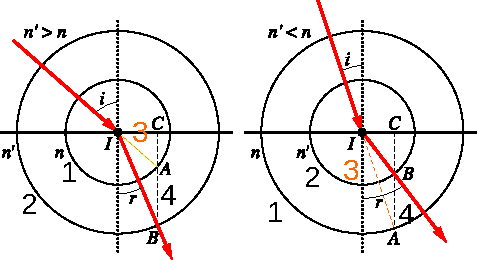
\includegraphics{fig1}
\subsection{Étude du prisme}
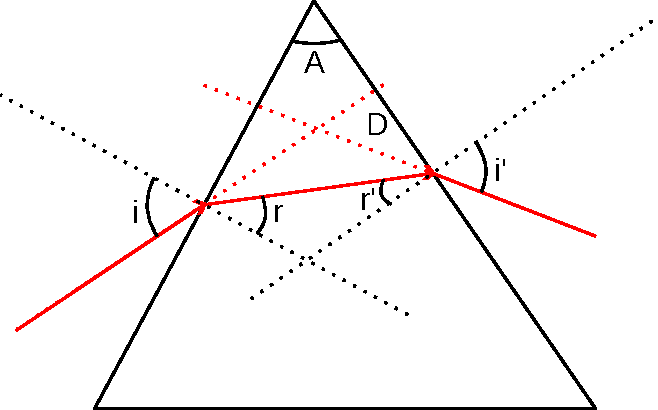
\includegraphics[scale=0.4]{prisme_1}
\subsubsection{Les 4 relations fondamentales}
On utilise les lois de Snell-Descartes pour trouver les 2 premières :
\begin{enumerate}
	 \item \(\sin(i) = n\sin(r)\)
	 \item \(\sin(i') = n\sin(r')\)
	\end{enumerate}
	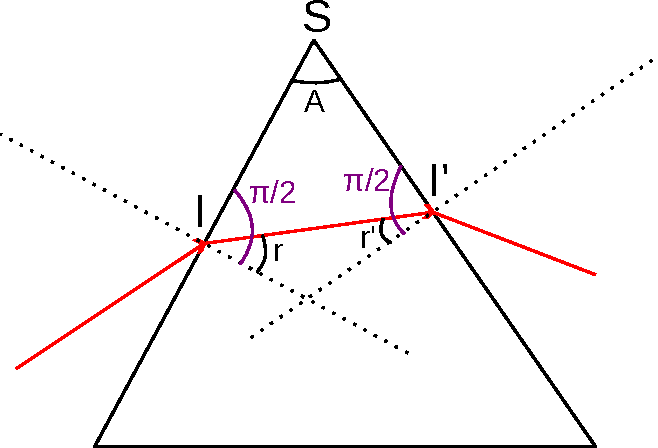
\includegraphics[scale=0.4]{prisme_2}

	On se place dans le triangle $SII'$ en appliquant la propriété de somme des angles d'un triangle. On a : \( \pi = A + (\frac{\pi}{2}-r) + (\frac{\pi}{2}-r')\), soit :
	\begin{enumerate}
	\setcounter{enumi}{2}
	 \item \(A = r+r'\)
	\end{enumerate}
	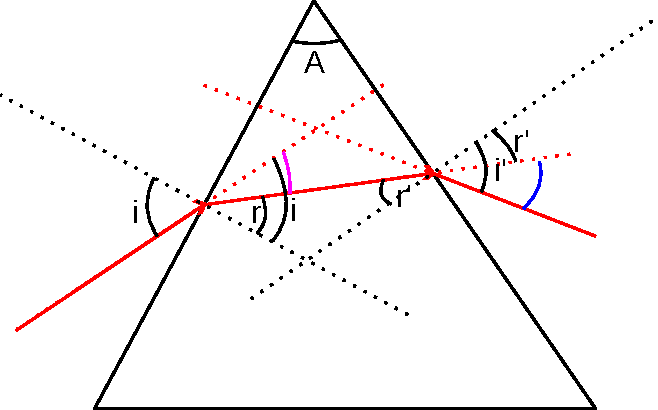
\includegraphics[scale=0.4]{prisme_3}

	On calcule la déviation totale pour trouver la dernière relation. \(D = {\color{purple}i-r} + {\color{blue}i'-r'}\), soit en replaçant les angles $r$ par $A$ :
	\begin{enumerate}
	\setcounter{enumi}{3}
	 \item \(D = i + i' - A\)
	\end{enumerate}
\subsubsection{Calcul de l'angle limite}
On cherche l'angle limite $i_{lim}$ pour observer un rayon en sortie du prisme. Pour pouvoir le voir, l'angle de sortie doit \^etre inférieur à $\frac{\pi}{2}$. Pour trouver $i_{lim}$, on prendra donc $i'=\frac{\pi}{2}$.
\explanation{ok_1}{On utilise la formule 3}
\explanation{ok_15}{L'expression précédente comporte $r'$. On va donc exprimer $r'$ en fonction de $i'$}
\explanation{ok_16}{En effet, $\sin(\frac{\pi}{2}) = 1$}
\explanation{ok_2}{On remplace $r'$ par son  expression}

\begin{flalign*}
\sin(i) &= n\sin(r)\\
&= n\sin(A-r')\explain{ok_1}{right}{0}{0.5}{}\\
&\\
\sin(i') &= n \sin(r')\explain{ok_15}{right}{0}{0.5}{}\\
1 &= n\sin(r')\explain{ok_16}{right}{0}{0.5}\\
r' &= \sin^{-1}(\frac{1}{n})\\
&\\
\sin(i) &= n\sin(A-\sin^{-1}(\frac{1}{n}))\explain{ok_2}{right}{0}{0.5}{}\\
i_{lim} &= \sin^{-1}(n\sin(A-\sin^{-1}(\frac{1}{n})))
\end{flalign*}
\subsubsection{Mesure de $n$ avec l'angle de déviation total minium}
On veut obtenir une valeur de $n$ par des mesures expérimentales. On conna\^it l'angle A avec précision. On va utiliser $D_m$ l'angle de déviation minimum, où l'on remarque que $i=i'=i_{min}$. On peut donc écrire $D_m = i+i'-A = 2i_{min} - A$, d'où $i_{min} = \frac{D_m+A}{2}$

On peut aussi simplifier l'expression 3 car si $i'=i, r'=r=r_{min}$. On obtient alors $r_{min} = \frac{A}{2}$.

En appliquant la loi de Snell-Descartes et replaçant $r_{min}$ et $i_{min}$ par leur expressions, on trouve : \(\sin(\frac{D_m+A}{2}) = n\sin(\frac{A}{2}) \) d'où l'on peut déduire $n$ : \(n=\frac{sin(\frac{D_m+A}{2}}{\sin(\frac{A}{2})}\).
\subsubsection{Calcul de $D_m$}
On souhaite déterminer la déviation $D$ en fonction de $n$ et de l'angle du rayon incident.

On utilise la 4e relation : $D = i+i'-A$. On ne connait pas $i'$, il va donc falloir l'exprimer en fonction de $A$ et $i$.

\begin{flalign*}
\sin(i')&=n\sin r'\\
&= n\sin(A-r)\\
&= n\sin(A- \sin^{-1}(\frac{\sin(i)}{n}) )
\end{flalign*}
On a plus qu'à remplacer $i'$ par son expression pour trouver $D$.
\subsection{Étude de l'arc-en-ciel}
\subsubsection{Analyse}
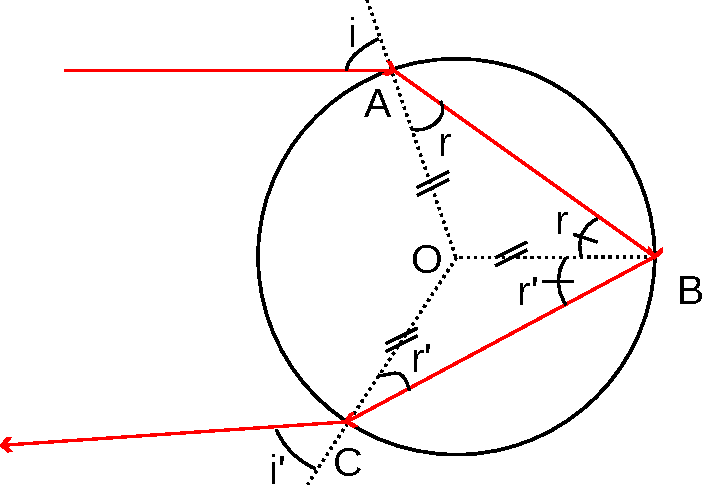
\includegraphics[scale=0.4]{goutte_1}

Les triangles ABO et OBC sont isocèles en O. On en déduit que les angles OAB et OBO sont égaux, tous commes les angles OBC et OCB. De plus, au point B la lumière est réflechie, donc d'après les propriétés de réflexion, OBC = OBO. On en déduit que r=r'.
\subsubsection{Angles de déviation total}
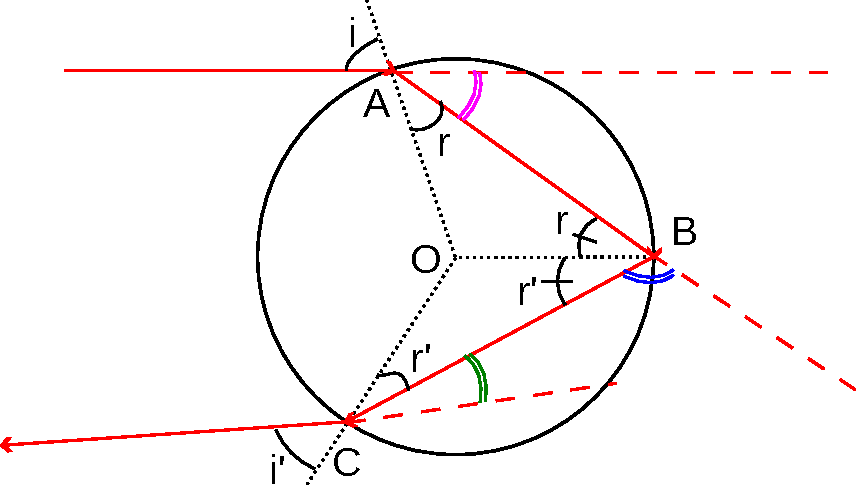
\includegraphics[scale=0.4]{goutte-2}

On cherche à exprimer l'angle de déviation total. On somme les angles des trois déviations : $D = {\color{purple}(i-r)} + {\color{blue}(\pi - 2r)} + {\color{ForestGreen}(i'-r)} = 2i + \pi -4r$
\subsubsection{Minimum de déviation}
On cherche l'angle $i$ pour lequel $D$ est minium, c'est-à-dire de dérivée nulle. On a donc $D'= 0 = 2 - 4\frac{\mathrm{d}r}{\mathrm{d}i} = 1-2\frac{\mathrm{d}r}{\mathrm{d}i}$

Il faut savoir que $\frac{\mathrm{d}r}{\mathrm{d}i} = \frac{\cos(i)}{n\cos(r)} =  \frac{\sqrt{1-\sin^2(i)}}{n\sqrt{1-\sin^2(r)}}$.

On obtient
\begin{flalign*}
1 &= 2\frac{\sqrt{1-\sin^2(i)}}{n\sqrt{1-\sin^2(r)}} = 2 \frac{\sqrt{1-\sin^2(i)}}{\sqrt{n^2-\sin^2(i)}}\\
&\iff \sqrt{n^2-\sin^2(i)} = 2\sqrt{1-\sin^2(i)}\\
&\iff n^2-\sin^2(i) = 4(1-\sin^2(i))\\
&\iff n^2-\sin^2(i) = 4-4\sin^2(i))\\
&\iff n^2 = 4-3\sin^2(i))\\
&\iff n^2-4=-3\sin^2(i))\\
&\iff i = \sin^{-1}(\sqrt{\frac{4-n^2}{3}})\\
\end{flalign*}
\subsubsection{Indice optique et couleur réfléchie}
Par la loi de Cauchy, on sait que si la longueur d'onde augmente, l'indice optique $n$ diminue. Or, $i_{lim}$ dépend de $n$, qui est soustrait. Ainsi, $i_{lim}$ augmente, ce qui fait diminuer $D_m$.

Cela explique pourquoi le rouge, avec une longueur d'onde plus grande,  est moins dévié que le bleu.


\end{document}

